\documentclass[a5paper]{report}
%\documentclass[a5paper,10pt]{scrartcl}

\usepackage[utf8]{inputenc}
\usepackage{geometry}
\usepackage{german}
\usepackage[pdftex]{graphicx}
\usepackage[fleqn]{amsmath}
\usepackage{amssymb}
\usepackage{amstext}
\usepackage{amsfonts}
\usepackage{mathrsfs}
\usepackage{hyperref}
\usepackage{color}
\usepackage{colortbl}
\usepackage{tabularx}
\usepackage{multicol}
\usepackage{rotating}

\title{Formelsammlung - ET/TI}
\author{Marc Ludwig}
\date{\today}

\pdfinfo{%
  /Title    (Formelsammlung - ET/TI)
  /Author   (Marc Ludwig)
  /Creator  (Marc Ludwig)
  /Producer (Marc Ludwig)
  /Keywords (Hilfe; Formeln; Hirn leer;...)
}

\hypersetup{linktocpage=true, colorlinks=false}	%Ganzseitiganzeigen %pdfpagemode=FullScreen,
\geometry{left=15mm,right=5mm, top=15mm, bottom=15mm}
\pagestyle{headings}
\hyphenation{words}
\allowdisplaybreaks

%Definitionen
\newcommand{\N}{\mathbb{N}}	%Natürliche Zahlen
\newcommand{\R}{\mathbb{R}}	%Reelle Zahlen
\newcommand{\C}{\mathbb{C}}	%Komplexe Zahlen


%%%%%%%%%%%%%%%Matzes Anpassungen

%Abstand zwischen Formeln
\setlength{\abovedisplayskip}{3mm}
\setlength{\belowdisplayskip}{3mm}

\newenvironment{merkbox}{\begin{minipage}{\linewidth}}{\end{minipage}}

%Einheitenbeschreibung
\newcommand{\des}[3][1]{$\left[#2\right]=\si{#1}$: {\small\textcolor{gray}{ #3}}}
\newcommand{\destext}[1]{{\small\textcolor{gray}{ #1}}}

\newcommand{\hebox}[1]{#1}
\newcommand{\heboxc}[1]{#1}

%Differential
\newcommand*\diff{\mathop{}\!\mathrm{d}}
\newcommand*\grad{\mathop{}\!\mathrm{grad}}
%%%%%%%%%%%%%%%%%%%%%%%%%%%%%%%%%%


\begin{document}
\maketitle

%INHALTSVERZEICHNIS
	\tableofcontents

		%TEIL
	\part{Mathematik}

	
		%KAPITEL
		\chapter{Algebra}
		
				%1. Abschnitt
	\section{Rechenregeln fuer Potenzen}
				
			
			\begin{align*}
				a^m \cdot a^n &= a^{m+n}	& \frac{a^m}{a^n} &= a^{m-n}	\\ \\
				\left( a^m \right)^n = \left( a^n \right)^m &= a^{m \cdot n} & a^n \cdot b^n &= \left( a \cdot b \right)^n	\\ \\
				\frac{a^n}{b^n} &= \left( \frac{a}{b} \right)^n	\\ \\
				\text{(fuer a} > \text{0) } a^b &= e^{b \cdot \ln a}
			\end{align*}
	
	%2.Abschnitt
	\vspace{10mm}
	\section{Zusammenhang zwischen Wurzeln und Potenzen}
		
	
			
				\boxed{
				\text{Im Folgenden wird vorausgesetzt, dass alle Potenzen und Wurzeln existieren.}
				} 
			
			
			\begin{align*}
				\sqrt[n]{a} &= a^{\frac{1}{n}} & \sqrt[n]{a^m} &= a^{\frac{m}{n}} & \left(\sqrt[n]{a}\right)^m &= a^{ \frac{m}{n}}
			\end{align*}
	
	%3.Abschnitt
	\newpage
	\section{Potenzen und Logarithmen}
	
	
			\text{Schreibweise: }
			x\(=\log_a \left(b\right) \text{ mit } a > 0, a \neq 1 \text{ und } b > 0 \text{.}\)
			\newline
			\text{Es gillt: }
			\(\log_a \left(1\right) = 0, \text{ } \log_a \left( a \right) = 1\)
			\text{.}
				
	%Unterpunkt
	\vspace{10mm}
	\subsection{Der natuerliche Logarithmus}
	
	
			%Hier muss der Limes noch angepasst werden, so dass der BEreich unter dem Ausdruck steht!
			\begin{flushleft}
			\text{Der Logarithmus zur Basis } \(e\) \text{ mit } \(e = \lim\limits_{n\to\infty} {\left(1+\frac{1}{n}\right)^n} = 2,71828...\)
			\begin{align*}
				\log_e \left(b\right) &= \ln \left(b\right) & \ln \left( \frac{1}{e} \right) = -1 ; \text{ da } e^{-1} = \frac{1}{e}
			\end{align*}
			
			\boxed{\text{Man beachte: } \text{x}^a = e^{\ln \left(\text{x}\right) \cdot a}}
			\end{flushleft}
	
	%Unterpunkt
	\vspace{10mm}
	\subsection{Rechnen mit Logarithmen}
	
	
			
			
			%Tabelle anlegen
			\begin{table}[h]
						
			\begin{tabular}{|l|l|}
				
				\hline
					\text{Es gillt:}
				&	%Dient als Ueberschrifft
					\text{Weitere Beziehungen:}
				\\
				\hline
					%Beginnt in der ersten Spalte, erste Zeile
   				\(\log_a \left({u \cdot v}\right) = \log_a \left(u\right) + \log_a \left(v\right)\)
				&	%In die naechste Spalte springen
					\( \log_a \left( \sqrt[n]{u} \right) = \frac{1}{n} \log_a \left( u \right)\)
				\\%Zurueck in die erste Spalte, zweite Zeile
					\(\log_a \left( \frac{u}{v} \right) = \log_a \left(u\right) - \log_a \left(v\right)\)
				&	%%In die naechste Spalte springen						
 					\(a^{\log_a \left(u\right)} = \log_a \left(a^u\right) = u\)
				\\%Zurueck in die erste Spalte, dritte Zeile
					\(\log_a \left(u^p\right) = p \cdot \log_a \left(u\right)\)
				&	%%In die naechste Spalte springen
					\(\log_a\left(u\right) = \frac{\log_c \left( u \right)}{\log_c \left( a \right)}\)
				\\
				%Unterstreicht die Tabelle
					\hline
								
			\end{tabular}
			\end{table}
			
	%4.Abschnitt
	\vspace{10mm}
	\section{Der Binomische Lehrsatz}
	
			
		Die Potenzen eines Binoms a+b lassen sich nach dem Binomischen Lehrsatz 
		\newline 
		wie folgt entwickeln \( \left(n \in \N^* \right)\):
		\vspace{5mm}
		\newline
		\( \left( a + b \right)^n = a^n + \binom{n}{1} a^{n-1} \cdot b^1 + \binom{n}{2} a^{n-2} \cdot b^2 + \binom{n}{3} a^{n-3} \cdot b^3 + 
		\ldots + \binom{n}{n-1} a^{1} \cdot b^{n-1} + b^n \)
		\vspace{5mm}
		\newline
		\text{Die Koeffizienten \( \binom{n}{k} \) heißen Binominalkoeffizienten, ihr Bildungsgesetz lautet:}
		\vspace{5mm}
		\newline
		\( \binom{n}{k} = \frac{n \left( n - 1 \right) \left( n - 2 \right) \ldots \left[ n - \left( k - 1 \right) \right]}{k!} = \frac{n!}{k! \left( n - k \right) !} \)
	
	\vspace{10mm}
	\subsubsection{Einige Eigenschaften der Binominalkoeffizienten}
		
		
			\begin{align*}
				\binom{n}{0} &= \binom{n}{n} = 1 & \binom{n}{k} &= 0 \text{ fuer k} > \text{n} & \binom{n}{1} &= \binom{n}{n-1} = n
				\\
				\binom{n}{k} &= \binom{n}{n-k} & \binom{n}{k} &+ \binom{n}{k+1} = \binom{n+1}{k+1}
			\end{align*}
			
	\vspace{10mm}
	\section{Sinus, Kosinus, Tangens und Kotangens}
	
	%Unterpunkt
	\vspace{10mm}
	\subsection{Beziehungen zwischen Sinus, Kosinus, Tangens und Kotangens}
	
	
		\begin{align*}
			&\sin^2 \left( \alpha \right) + \cos^2 \left( \alpha \right) = 1 & &\tan \left( \alpha \right) \cdot \cot \left( \alpha \right) = 1	
			\\
			&\tan \left( \alpha \right) = \frac{\sin \left( \alpha \right)}{\cos \left( \alpha \right)} & &\cot \left( \alpha \right) = \frac{\cos \left( \alpha \right)}{\sin \left( \alpha \right)} 
			\\
			&1 + \tan^2 \left( \alpha \right) = \frac{1}{\cos^2 \left( \alpha \right)} & &1 + \cot^2 \left( \alpha \right) = \frac{1}{\sin^2 \left( \alpha \right)}
		\end{align*}
	
	%Unterpunkt	
	\vspace{10mm}
	\subsection{Additionstheoreme}
	
	
		\begin{align*}
			\sin \left( \alpha \pm \beta \right) &= \sin \left( \alpha \right) \cos \left( \beta \right) \pm \cos \left( \alpha \right) \sin \left( \beta \right)
			\\ 
			\cos \left( \alpha \pm \beta \right) &= \cos \left( \alpha \right) \cos \left( \beta \right) \mp \sin \left( \alpha \right) \sin \left( \beta \right)
			\\
			\tan \left( \alpha \pm \beta \right) &= \frac{\tan \left( \alpha \right) \pm \tan \left( \beta \right)}{1 \mp \tan \left( \alpha \right) \tan \left( \beta \right)}
		\end{align*}
		
	%Unterpunkt
	\vspace{10mm}
	\subsection{Funktionen des doppelten und halben Winkels}
			
			
			\begin{align*}
				\sin \left( 2 \alpha \right) &= 2 \sin \left( \alpha \right) \cos \left( \alpha \right) 
				\\
				\cos \left( 2 \alpha \right) &= \cos^2 \left( \alpha \right) - \sin^2 \left( \alpha \right) = 2 \cos^2 \left( \alpha \right) -1 = 1 - 2 \sin^2 \left( \alpha \right)
				\\
				\tan \left( 2 \alpha \right) &= \frac{2 \tan \left( \alpha \right)}{1 - \tan^2 \left( \alpha \right)}
				\\
				\sin^2 \left( \frac{\alpha}{2} \right) &= \frac{1}{2} \left( 1 - \cos \left( \alpha \right) \right)
				\\
				\cos^2 \left( \frac{\alpha}{2} \right) &= \frac{1}{2} \left( 1 + \cos \left( \alpha \right) \right)
				\\
				\tan^2 \left( \frac{\alpha}{2} \right) &= \frac{1 - \cos \left( \alpha \right)}{1 + \cos \left( \alpha \right)}
			\end{align*}
			
	%Unterpunkt
	\vspace{10mm}
	\subsection{Umformungen}
	
	%Unterunterpunkt :)
	\vspace{10mm}
	\subsubsection{Summe oder Differenz in ein Produkt}
	
	
			\begin{flushleft}
				\(\sin \left( \alpha \right) + \sin \left( \beta \right) = 2 \sin \left( \frac{\alpha + \beta}{2}\right) \cos \left( \frac{\alpha - \beta}{2} \right)\)
				\\
				\(\sin \left( \alpha \right) - \sin \left( \beta \right) = 2 \cos \left( \frac{\alpha + \beta}{2}\right) \sin \left( \frac{\alpha - \beta}{2} \right)\)
				\\
				\(\cos \left( \alpha \right) + \cos \left( \beta \right) = 2 \cos \left( \frac{\alpha + \beta}{2}\right) \cos \left( \frac{\alpha - \beta}{2} \right)\)
				\\
				\(\cos \left( \alpha \right) - \cos \left( \beta \right) = -2 \sin \left( \frac{\alpha + \beta}{2}\right) \sin \left( \frac{\alpha - \beta}{2} \right)\)
			\end{flushleft}
	
	%Unterunterpunkt :)
	\vspace{10mm}
	\subsubsection{Produkt in eine Summe oder Differenz}
	
	
			\begin{flushleft}
				\(2 \sin \left( \alpha \right) \sin \left( \beta \right) = \cos \left( \alpha - \beta \right) - \cos \left( \alpha + \beta \right)\)
				\\
				\(2 \cos \left( \alpha \right) \cos \left( \beta \right) = \cos \left( \alpha - \beta \right) + \cos \left( \alpha + \beta \right)\)
				\\
				\(2 \sin \left( \alpha \right) \cos \left( \beta \right) = \sin \left( \alpha - \beta \right) + \sin \left( \alpha + \beta \right)\)
			\end{flushleft}
	
	%5.Abschnitt		
	\vspace{10mm}	
	\section{Komplexe Zahlen}
			
			
			\text{Für die Menge aller komplexen Zahlen schreibt man:}
			\vspace{5mm}
			\\
			\fbox{\( \C = \left\{ z | z = a + bj, a \in \R \wedge b \in \R \right\} \)}
			\vspace{5mm}
			\\
			\text{a-Realteil \ \  b-Imaginaerteil \ \  j-imaginaere Einheit}
			
			
			%Tabelle
			\begin{table}[h]
			
				\begin{tabular}{|l|l|l|}
				\hline
 				\text{kartesiche Form} & \text{trigonometrische Form}  & \text{exponentialform}	 \\ 
				\hline
 				\( z = a + bj \) & \( z = \left| z \right| \left( \cos \varphi + j \cdot \sin \varphi \right) \)  & \( z = \left| z \right| \cdot e^{j 	\varphi} \)  \\ 
				\hline
 				\( z^* = \left( a + bj \right)^* = a-bj \) & \( z^* = \left| z \right| \left( \cos \varphi - j \cdot \sin \varphi \right) \) & \( z^* = \left| z \right| \cdot e^{-j \varphi} \) \\ 
				\hline
				\end{tabular}
			
			\end{table}
			
			\begin{flushleft}
				\text{\( \left| z \right| \) = Betrag von z}
				\\
				\text{\( \varphi \) = Argument (Winkel) von z}
				\\
				\text{\( z^* \) = Konjugiert komplexe Zahl}
			\end{flushleft}
			
		%Unterpunkt
		\vspace{10mm}
		\subsection{Umrechnungen zwischen den Darstellungsformen}
			
			\vspace{10mm}
			\subsubsection{Polarform \(\rightarrow\) Kartesiche Form}
			
			
				\( z = \left| z \right| \cdot e^{j \varphi} = \left| z \right| \left( \cos \varphi + j \cdot \sin \varphi \right) = 
				\underbrace{\left| z \right| \cdot \cos \varphi}_{a} + j \cdot \underbrace{\left| z \right| \cdot \sin \varphi}_{b} = a + bj \)	
			
			\vspace{10mm}
			\subsubsection{Kartesische Form \(\rightarrow\) Polarform}
			
			
				\( \left| z \right| = \sqrt{a^2 + b^2}\), \ \ \(\tan \varphi = \frac{b}{a} \)
				
		%Unterpunkt
		\vspace{10mm}
		\subsection{Rechnen mit Komplexen Zahlen}
		
			\vspace{10mm}
			\subsubsection{Multiplikation}
								
				
				\fbox{In kartesischer Form:}
								
				\begin{center}
				\(z_1 \cdot z_2 = \left( a_1 + j b_1 \right) \cdot \left( a_2 + j b_2 \right) 
												= \left( a_1 a_2 - b_1 b_2 \right) + j \cdot \left( a_1 b_2 + a_2 b_1 \right)\)
				\end{center}
								
				\fbox{In der Polarform:}
												
				\begin{align*}
					z_1 \cdot z_2 &= \left[ \left| z_1 \right| \left( \cos \varphi_1 + j \cdot \sin \varphi_1 \right) \right] \cdot 
													 \left[ \left| z_2 \right| \left( \cos \varphi_2 + j \cdot \sin \varphi_2 \right) \right]
					\\
					&= \left( \left| z_1 \right| \left| z_2 \right| \right) \cdot \left[ \cos \left( \varphi_1 + \varphi_2 \right) +  
					j \cdot \sin \left(	\varphi_1 + \varphi_2 \right) \right]
					\\
					&= \left( \left| z_1 \right| \cdot e^{j \varphi_1} \right) \cdot \left( \left| z_2 \right| \cdot e^{j \varphi_2} \right)
					= \left( \left| z_1 \right| \left| z_2 \right| \right) \cdot e^{j \left( \varphi_1 + \varphi_2 \right)}
				\end{align*}
			
			\vspace{10mm}	
			\subsubsection{Division}
			
				\fbox{In kartesischer Form}
				
					\begin{center}
						
					\end{center}
				
				\fbox{In der Polarform}
		
		\chapter{Lineare Algebra}

			Ein Test um das Skript auszuprobieren.

	%Physik als eigenes Dokument, mit eigenen *.tex Files
	\part{Physik}
	
		\chapter{Kinematik}
		\begin{quote}
Perfection is achieved\\only on the point of collapse.\\- C. N. Parkinson
\end{quote}

\section{Analogietabelle}
\index{Kinematik!Analogietabelle Translation - Rotation}

%Wegen Build Fehlern, ein '\:' vor jedem '\downarrow' entfernt

\begin{center}
\begin{tabular}{l|l|l}
\text{Translation} &  & \text{Rotation}\\\hline
\(\vec{s}\) &  & \(\vec{\varphi}\)\\
\(\downarrow\frac{ds}{dt}\) &  & \(\downarrow \frac{d\varphi}{dt}\)\\
\(\vec{v}\) & \(\vec{v}=\vec{\omega} \times \vec{r}\) & \(\vec{\omega}\)\\
\(\downarrow\frac{dv}{dt}\) &  & \(\downarrow \frac{d\omega}{dt}\)\\
\(\vec{a}\) & \(a = \underbrace{\alpha \times r}_{a_{Tan}} - \underbrace{\omega^2 r}_{a_R}\) & \(\vec{\alpha}\)\\\hline
m &  & J\\
\(\downarrow \frac{dm}{dt}\) &  & \(\downarrow \frac{dJ}{dt}\)\\
\(\vec{F}\) &  & \(\vec{M}\)\\
\(\downarrow \frac{dF}{dt}\) &  & \(\downarrow \frac{dM}{dt}\)\\
\(\vec{p}\) &  & \(\vec{L}\)\\
\(\frac{m}{2}v^2\) & \(E_{kin}\) & \(\frac{J}{2}\omega^2\)
\end{tabular}
\end{center}

\newpage
\begin{multicols}{2}{}
\subsection{Translation}
\index{Kinematik!Translation}
\begin{align*}
	a(t)&=a_0=\frac{\diff v}{\diff t}=\dot{v}=\ddot{s} \\
	v(t)&=a_0\cdot t+v_0=\frac{\diff s}{\diff t}=\dot{s} \\
	s(t)&=\frac{1}{2}a_0\cdot t^2+v_0\cdot t+s_0
\end{align*}

\subsection{Rotation}
\index{Kinematik!Rotation}
\begin{align*}
\alpha(t)&=\alpha_0=\frac{\diff \omega}{\diff t}=\dot{\omega}=\ddot{\varphi} \\
\omega(t)&=\alpha_0\cdot t+\omega_0=\frac{\diff \varphi}{\diff t}=\dot{\varphi} \\
\varphi(t)&=\frac{1}{2}\alpha_0\cdot t^2+\omega_0\cdot t+\varphi_0
\end{align*}
\end{multicols}

\begin{multicols}{2}{}
\subsubsection*{Bahngroessen}
\index{Kinematik!Bahngrößen}
\begin{align*}
a_t(t)&=a_0=\frac{\diff v}{\diff t}=\dot{v}=\ddot{s} \\
v(t)&=a_0\cdot t+v_0=\frac{\diff s}{\diff t}=\dot{s} \\
s(t)&=\frac{1}{2}a_0\cdot t^2+v_0\cdot t+s_0
\end{align*}


\subsubsection*{Winkelgroessen}
\index{Kinematik!Winkelgrößen}
\begin{align*}
\vec{a_t}	&=\vec{\alpha} \times \vec{r} =\alpha\cdot r \qquad \alpha \perp r \\
\vec{\alpha}	&=\vec{r} \times \vec{a_t}\\
\vec{v}		&=\vec{\omega}\times\vec{r} =\omega\cdot r  \qquad \omega \perp r\\
\vec{\omega}	&=\vec{r} \times \vec{v}\\
s		&=\varphi\cdot r  
\end{align*}
\end{multicols}        


\begin{multicols}{2}{}
\subsubsection*{Kreisfrequenz}
\begin{align*}
\omega&=\frac{2\cdot\pi}{T}\\
&=2\cdot\pi\cdot n \\
&=2\cdot\pi\cdot f
\end{align*}


\subsubsection*{Radialbeschleunigung}
\begin{align*}
a_r&=\frac{v^2}{r}\\
&=v\cdot\omega\\
&=\omega^2\cdot r
\end{align*}
\end{multicols}


\subsubsection*{Umdrehungen}
\begin{align*}
N&=\frac{\omega_0\cdot t}{2\cdot \pi}+\frac{1}{2}\cdot\frac{\alpha}{2\cdot \pi}\cdot t^2\\
&=n_0\cdot t+\frac{\alpha}{4\cdot\pi}\cdot t^2
\end{align*}


\newpage
\section{Dynamik}

\subsection{Geradlinig (Translation)}
\begin{align*}
\vec{F}&=m\cdot \vec{a}\\
\vec{F}_{\text{Tr}}&=-m\cdot \vec{a}
\end{align*}
\begin{multicols}{2}{}
\subsubsection*{Impuls}
\index{Translation!Impuls}
\begin{align*}
\vec{p}&=m\cdot \vec{v}\\ \\
\end{align*}

\subsubsection*{Kraftstoss}
\begin{align*}
\vec{F}&=\frac{\diff \vec{p}}{\diff t}=m\cdot\frac{\diff \vec{v}}{\diff t}+\vec{v}\cdot\frac{\diff m}{\diff t}\\
\Delta\vec{p}&=\vec{p}_2-\vec{p}_1=\int_{\vec{p}_2}^{\vec{p}_1}\diff p=\int_0^{t}\vec{F}\diff t
\end{align*}
\end{multicols}

\begin{multicols}{2}{}
\subsubsection*{Arbeit}
\index{Translation!Arbeit}
\begin{align*}
W&=-\int_{\vec{s}_1}^{\vec{s}_2}\vec{F_{\text{Tr}}}\circ\diff \vec{s}\\
&=\int_{\vec{v}_0}^{\vec{v}_1}m\vec{v}\circ\diff \vec{v}=\frac{1}{2}m\left(v_1^2-v_0^2\right) 
\end{align*}

\subsubsection*{Hubarbeit}
\begin{align*}
W_{\text{hub}}&=mgh
\end{align*}
\end{multicols}

\begin{multicols}{2}{}
\subsubsection*{Kinetische Energie}
\begin{align*}
E_{\text{kin}}=\frac{1}{2}mv^2
\end{align*}

\subsubsection*{Leistung}
\begin{align*}
P=\vec{F}\circ\vec{v}=\frac{\diff W}{\diff t}=\dot{W}
\end{align*}
\end{multicols}


\subsection{Drehbewegung(Rotation)}
\begin{multicols}{2}{}
\subsubsection*{Massentraegheitsmoment}
\index{Rotation!Massenträgheitsmoment}
\begin{align*}
J=\int r^2 \diff m
\end{align*}

\subsubsection*{Drehmoment}
\index{Rotation!Drehmoment}
\begin{align*}
\vec{M}&=\vec{r}\times\vec{F}=J\vec{\alpha}=\dot{\vec{L}}
\end{align*}
\end{multicols}

\begin{multicols}{2}{}
\subsubsection*{Drehimpuls}
\index{Rotation!Drehimpuls}
\begin{align*}
\vec{L}&=\vec{r}\times\vec{p} \\
&=J\cdot \vec{\omega}
\end{align*}

\subsubsection*{Kinetische Energie}
\begin{align*}
E_{kin}=\frac{1}{2}J\omega^2 \\
\end{align*}
\end{multicols}

\begin{multicols}{2}{}
\subsubsection*{Arbeit}
\begin{align*}
W &=\int_{\varphi_0}^{\varphi_1}\vec{M}\circ\vec{e_\omega}\diff \varphi \\
&=\int_{\vec{\omega}_0}^{\vec{\omega}_1}J\vec{\omega}\diff\vec{\omega}\\
&=\frac{1}{2}J\left(\omega_1^2-\omega_0^2\right)
\end{align*}

\subsubsection*{Leistung}
\begin{align*}
P=\vec{M}\circ\vec{\omega}
\end{align*}

\subsubsection*{Zentripedalkraft}
\index{Rotation!Zentripedalkraft}
\begin{align*}
F_{zp}&=-m\cdot\omega^2\cdot r\\
&=-m\cdot v^2\cdot \frac{\vec{e_r}}{r}
\end{align*}
\end{multicols}


\subsection{Geneigte Ebene}
\index{Geneigte Ebene}
\subsubsection*{Kräfte}
\begin{align*}
\vec{F}_N&=\vec{F}_G\cos\alpha\\
\vec{F}_H&=\vec{F}_G\sin\alpha
\end{align*}


\subsection{Reibung}

\begin{multicols}{2}{}
\subsubsection*{Reibungskraft}
\begin{align*}
F_R=\mu\cdot F_N
\end{align*}
\vfill
\subsubsection*{Rollreibung}
\begin{align*}
M&=f\cdot F_N\\
F_R&=\frac{f}{r}\cdot F_N
\end{align*}
\vfill
\end{multicols}

\newpage
\subsection{Feder}
\begin{multicols}{2}{}
\subsubsection*{HOOKsches Gesetz}
\index{Hook'sches Gesetz}
\begin{align*}
F&=-kx\\
M&=D\varphi
\end{align*}

\subsubsection*{Federspannarbeit}
\begin{align*}
W	&=\int_{x_\text{min}}^{x_\text{max}}F\diff x=\int_{x_\text{min}}^{x_\text{max}}kx\diff x\\
	&=\frac{1}{2}\cdot k\cdot \left(x_{\text{max}}^2-x_{\text{min}}^2\right)
\end{align*}
\end{multicols}

\subsection{Elastischer Stoß}
\begin{align*}
\text{Energie vor den Stoß} &= \text{Energie nach den Stoß}\nonumber\\
\sum E_{\text{kin}}&=\sum E_{\text{kin}}'
\end{align*}


\subsubsection*{Impulserhaltung}
\index{Elastischer Stoß!Impulserhaltung}
\begin{align*}
\text{Impuls vor den Stoß} &= \text{Impuls nach den Stoß}\nonumber\\
\sum m\vec{v}&= \sum m\vec{v}'
\end{align*}


\subsubsection*{Zentraler, Gerader, Elastischer Stoß}
\index{Elastischer Stoß!Zentral und Gerade}
\begin{align*}
\frac{1}{2}m_1v_1^2+\frac{1}{2}m_2v_2^2&=\frac{1}{2}m_1v_1'^2+\frac{1}{2}m_2v_2'^2\\
m_1v_1+m_2v_2&=m_1v_1'+m_2v_2'
\end{align*}

\begin{align*}
v_2'&=\frac{2m_1}{m_1+m_2}v_1+\frac{m_2-m_1}{m_1+m_2}v_2\\
v_1'&=\frac{2m_2}{m_1+m_2}v_2+\frac{m_1-m_2}{m_1+m_2}v_1
\end{align*}

\newpage
\subsection{Unelastischer Stoß}
\index{Unelastischer Stoß!Energieerhaltung}
\subsubsection*{Energieerhaltung}
\begin{align*}
\text{Energie vor den Stoß} &= \text{Energie nach den Stoß}+\text{Arbeit}\nonumber\\
\sum E_{\text{kin}}&=\sum E_{\text{kin}}'+\Delta W
\end{align*}


\subsubsection*{Impulserhaltung}
\index{Unelastischer Stoß!Impulserhaltung}
\begin{align*}
\text{Impuls vor den Stoß} &= \text{Impuls nach den Stoß}\nonumber\\
\sum m\vec{v}&= \sum m\vec{v}'
\end{align*}


\subsubsection*{Total unelastischer Stoss}
\begin{align*}
\frac{1}{2}m_1v_1^2+\frac{1}{2}m_2v_2^2&=\frac{1}{2}\left(m_1+m_2\right)v'^2+\Delta W\\
m_1v_1+m_2v_2&=\left(m_1+m_2\right)v'
\end{align*}

\begin{align*}
v'&=\frac{m_1v_1+m_2v_2}{m_1+m_2}
\end{align*}

\begin{align*}
\Delta W	&=\frac{m_1\cdot m_2}{2\left(m_1+m_2\right)}\left(v_1-v_2\right)^2
\end{align*}



\subsubsection*{Drehimpulserhaltungssatz}
\begin{align*}
\text{Drehinpuls zur Zeit 1} &= \text{Drehimpuls zur Zeit 2}\\
\sum \vec{L}&=\sum \vec{L}'
\end{align*}


\subsubsection*{Kopplung zweier Rotationskörper}
\begin{align*}
\vec{\omega}'&=\frac{J_0\vec{\omega_0}+J_1\vec{\omega_1}}{J_1+J_2}\\
W&=\frac{J_0\cdot J_1}{2\left(J_0+J_1\right)}\left(\omega_0-\omega_1\right)^2
\end{align*}


\subsection{Rotierendes Bezugssystem}
\index{Rotierendes Bezugssystem!Zentrifugalkraft}
\begin{multicols}{2}{}
\subsubsection*{Zentrifugalkraft}
\begin{align*}
\vec{F}_Z&=F_r\cdot \vec{e}_r=-m\vec{\omega}\times\left(\vec{\omega}\times\vec{r}\right)\\
&=-m\vec{\omega}\times\vec{v}\\
F_Z&=-m\frac{v^2}{r}=-m\omega^2 r
\end{align*}


\subsubsection*{Corioliskraft}
\index{Rotierendes Bezugssystem!Corioliskraft}
\begin{align*}
\vec{F}_C&=-2m\vec{\omega}\times\vec{v}
\end{align*}
\vspace{10mm}
\end{multicols}

\section{Schwerpunkt}
\index{Schwerpunkt!Punktmasse}
\begin{multicols}{2}{}
\subsection*{mehrere Punktmassen}
\begin{align*}
\vec{r}_{\text{Sp}}=\frac{\sum\vec{r}_i m_i}{\sum\ m_i}
\end{align*}


\subsection*{Allgemein}
\index{Schwerpunkt!Allgemein}
\begin{align*}
\vec{r}_{\text{Sp}}=\frac{\int \vec{r}\diff m}{\int \diff m}
\end{align*}
\end{multicols}

\begin{multicols}{2}{}
\subsubsection*{Schwerpunkt in \\Zylinderkoordinaten}
\index{Schwerpunkt!Zylinderkoordinaten}
\begin{align*}
r_{\text{Sp}}&=\frac{\int_z\int_\varphi\int_r r^2\rho \diff r \diff \varphi \diff z }{\int_z\int_\varphi\int_r r\rho \diff r \diff \varphi \diff z }\\
\varphi_{\text{Sp}}&=\frac{\int_z\int_\varphi\int_r \varphi r\rho \diff r \diff \varphi \diff z }{\int_z\int_\varphi\int_r r\rho \diff r \diff \varphi \diff z }\\
z_{\text{Sp}}&=\frac{\int_z\int_\varphi\int_r z r\rho \diff r \diff \varphi \diff z }{\int_z\int_\varphi\int_r r\rho \diff r \diff \varphi \diff z }\\
x&=r\cos{\varphi}\hspace{3mm}y=r\sin{\varphi}\hspace{3mm}z=z
\end{align*}

\subsubsection*{Schwerpunkt in \\karthesischen Koordinaten}
\index{Schwerpunkt!Kartesischekoordinaten}
\begin{align*}
x_{\text{Sp}}&=\frac{\int_z\int_y\int_x x\rho \diff x \diff y \diff z }{\int_z\int_y\int_x \rho \diff x \diff y \diff z }\\
y_{\text{Sp}}&=\frac{\int_z\int_y\int_x y\rho \diff x \diff y \diff z }{\int_z\int_y\int_x \rho \diff x \diff y \diff z }\\
z_{\text{Sp}}&=\frac{\int_z\int_y\int_x z\rho \diff x \diff y \diff z }{\int_z\int_y\int_x \rho \diff x \diff y \diff z }
\end{align*}
\hfill
\end{multicols}


\newpage
\section{Trägheitsmoment}
\index{Trägheitsmoment}
\begin{align*}
J&=\sum m_i r_i^2\\
J&=\int_m r^2 \diff m \\
J&=\int_z\int_\varphi\int_r r^3\rho \diff r \diff \varphi \diff z 
\end{align*}

\subsection*{}%Leer hmpf\ldots!

\begin{multicols}{2}{}
\subsubsection*{STEINER'scher Satz}
\begin{align*}
J_x&=mr^2+J_s
\end{align*}

%Tabelle einfügen
\subsubsection*{Trägheitsmoment Kugel}
\begin{align*}
J_\text{Sp}&=\frac{2}{5}mr^2
\end{align*}


\subsubsection*{Trägheitsmoment Zylinder}
\begin{align*}
J_\text{Sp}&=\frac{1}{2}mr^2
\end{align*}


\subsubsection*{Trägheitmoment Kreisring \\(Torus)}
\begin{align*}
J_\text{Sp}&=mr^2
\end{align*}


\subsubsection*{Trägheitsmoment Stab}
\begin{align*}
J_\text{Sp}=\frac{1}{12}ml^2
\end{align*}
\end{multicols}


\newpage
\section{Elastizitätslehre}
\subsection*{}%Leer hmpf\ldots!

\begin{multicols}{2}{}
\subsubsection*{Spannung}
\index{Elastizitätslehre!Spannung}
\begin{align*}
\vec{\sigma}&=\frac{\diff\vec{F}_n}{\diff A}\\
\sigma&=E \varepsilon=E\frac{\Delta l}{l}\\
\vec{\tau}&= \frac{\diff\vec{F}_t}{\diff A}
\end{align*}
\hfill

\begin{center}
 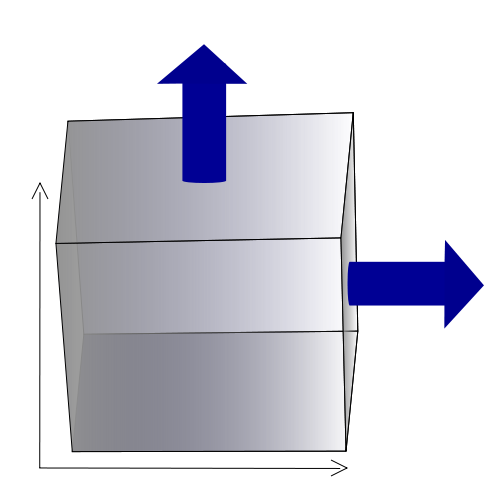
\includegraphics[width=40mm,height=40mm,keepaspectratio=true]{./Physik/Bilder/Spannung.png}
\end{center}
\end{multicols}


\subsubsection*{Schubmodul}
\index{Elastizitätslehre!Schub}
\begin{multicols}{2}{}
\begin{align*}
G&=\frac{\tau}{\varphi}
\end{align*}
\hfill

\begin{center}
 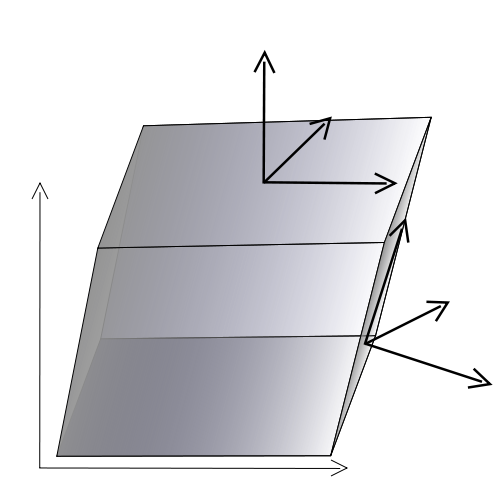
\includegraphics[width=40mm,height=40mm,keepaspectratio=true]{./Physik/Bilder/Tangentialspannung.png}
\end{center}
\end{multicols}


\subsubsection*{Drillung}
\index{Elastizitätslehre!Drill}
\begin{multicols}{2}{}
\begin{align*}
\psi&=\frac{\diff \varphi}{\diff l}=\frac{W_t}{G\cdot J_p}\tau=\frac{M_t}{G\cdot J_p}
\end{align*}
\hfill

\begin{center}
 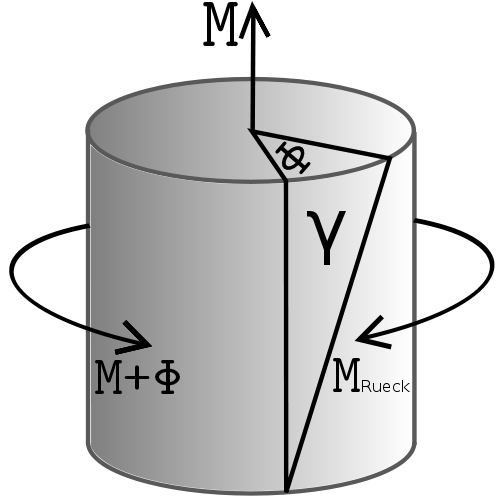
\includegraphics[width=40mm,height=40mm,keepaspectratio=true]{./Physik/Bilder/Scherbeanspruchung.png}
\end{center}
\end{multicols}


\begin{multicols}{2}{}
\subsubsection*{Flächenmoment}
\index{Elastizitätslehre!Flächenmoment}
\begin{align*}
J_p&=\int r^2\diff A=\int_\varphi\int_r r^3\diff r \diff \varphi 
\end{align*}


\subsubsection*{Verformungsarbeit}
\index{Elastizitätslehre!Verformungsarbeit}
\begin{align*}
W&=V\int \sigma(\varepsilon) \diff \varepsilon 
\end{align*}
\end{multicols}


\section{Schwingungen}
\subsection*{}%Leer hmpf\ldots!

\subsubsection*{Harmonische Schwingungen}
\begin{align*}
u(t)=A\cos(\omega t+\varphi_0)
\end{align*}


\subsection{Ungedämpfte Schwingungen}

\begin{align*}
\ddot{x}&=-\frac{k}{m}x\\
x(t)&=\hat{x}\cos(\omega_0 t+\varphi_0)\\
\dot{x}(t)&=-\hat{x}\omega\sin(\omega_0 t+\varphi_0)\\
\ddot{x}(t)&=-\hat{x}\omega^2\cos(\omega_0 t+\varphi_0)\\
\omega&=\sqrt{\frac{k}{m}}\\
f&=\frac{1}{2\pi}\sqrt{\frac{k}{m}}\\
T&=2\pi\sqrt{\frac{m}{k}}
\end{align*}

\newpage
\begin{multicols}{2}{}
\subsubsection*{Mathemetisches Pendel}
\index{Schwingungen!Mathematisches Pendel}
\begin{align*}
\ddot{\varphi}&=-\frac{g}{l}\varphi\\
\varphi(t)&=\hat{\varphi}\cos(\omega_0 t+\varphi_0)\\
\dot{\varphi}(t)&=-\hat{\varphi}\omega\sin(\omega_0 t+\varphi_0)\\
\ddot{\varphi}(t)&=-\hat{\varphi}\omega^2\cos(\omega_0 t+\varphi_0)\\
\omega&=\sqrt{\frac{g}{l}}\\
f&=\frac{1}{2\pi}\sqrt{\frac{g}{l}}\\
T&=2\pi\sqrt{\frac{l}{g}}
\end{align*}

\subsubsection*{Physikalisches Pendel}
\index{Schwingungen!Physikalisches Pendel}
\begin{align*}
\ddot{\varphi}&=-\frac{lmg}{J_A}\varphi\\
\varphi(t)&=\hat{\varphi}\cos(\omega_0 t+\varphi_0)\\
\dot{\varphi}(t)&=-\hat{\varphi}\omega\sin(\omega_0 t+\varphi_0)\\
\ddot{\varphi}(t)&=-\hat{\varphi}\omega^2\cos(\omega_0 t+\varphi_0)\\
\omega&=\sqrt{\frac{mgl}{J_A}}\\
f&=\frac{1}{2\pi}\sqrt{\frac{mgl}{J_A}}\\
T&=2\pi\sqrt{\frac{J_A}{mgl}}
\end{align*}
\end{multicols}

\begin{multicols}{2}{}
\subsubsection*{Torsionsschwingung}
\index{Schwingungen!Torsionsschwingung}
\begin{align*}
\ddot{\varphi}&=-\frac{D}{J_A}\varphi\\
\varphi(t)&=\hat{\varphi}\cos(\omega_0 t+\varphi_0)\\
\dot{\varphi}(t)&=-\hat{\varphi}\omega\sin(\omega_0 t+\varphi_0)\\
\ddot{\varphi}(t)&=-\hat{\varphi}\omega^2\cos(\omega_0 t+\varphi_0)\\
\omega&=\sqrt{\frac{D}{J_A}}\\
f&=\frac{1}{2\pi}\sqrt{\frac{D}{J_A}}\\
T&=2\pi\sqrt{\frac{J_A}{D}}
\end{align*}



\subsubsection*{Flüssigkeitspendel}
\index{Schwingungen!Flüssigkeitspendel}
\begin{align*}
\ddot{y}&=-\frac{2A\rho g}{m}y\\
\varphi(t)&=\hat{y}\cos(\omega_0 t+\varphi_0)\\
\dot{\varphi}(t)&=-\hat{y}\omega\sin(\omega_0 t+\varphi_0)\\
\ddot{\varphi}(t)&=-\hat{y}\omega^2\cos(\omega_0 t+\varphi_0)\\
\omega&=\sqrt{\frac{2A\rho g}{m}}=\sqrt{\frac{2g}{l}}\\
f&=\frac{1}{2\pi}\sqrt{\frac{2g}{l}}\\
T&=2\pi\sqrt{\frac{l}{2g}}
\end{align*}
\end{multicols}

\begin{multicols}{2}
\subsubsection*{Elektrischer Schwingkreis}
\begin{align*}
0&=L\ddot{Q}+\frac{Q}{C}\\
q(t)&=\hat{Q}\cos(\omega_0 t+\varphi_0)\\
\dot{q}(t)&=-\hat{Q}\omega\sin(\omega_0 t+\varphi_0)\\
\ddot{q}(t)&=-\hat{Q}\omega^2\cos(\omega_0 t+\varphi_0)\\
\omega&=\sqrt{\frac{1}{LC}}\\
f&=\frac{1}{2\pi}\sqrt{\frac{1}{LC}}\\
T&=2\pi\sqrt{\frac{1}{LC}}
\end{align*}
\vfill
\end{multicols}


\subsection{Gedämpfte Schwingungen}

\begin{multicols}{2}{}
\subsubsection*{Schwingungsgleichung}
\index{Schwingungen!gedämpft!Schwingungsgleichung}
\begin{align*}
m\ddot{x}=-kx+F_R
\end{align*}
\hfill

\subsubsection*{COULOMB Reibung}
\index{Schwingungen!gedämpft!COULOMB Reibung}
\begin{align*}
F_R&=-\operatorname{sgn}({\dot{x}})\mu F_N\\
0&=m\ddot{x}+kx+\operatorname{sgn}({\dot{x}})\mu F_N\\
\end{align*}
\end{multicols}


\subsubsection*{Gleitreibung}
\index{Schwingungen!gedämpft!Gleitreibung}
\begin{align*}
x(t)&=-(\hat{x}_0-\hat{x}_1)\cos(\omega t)-\hat{x}_1\qquad 0\leq t\leq \frac{T}{2}\\
x(t)&=-(\hat{x}_0-3\hat{x}_1)\cos(\omega t)+\hat{x}_1\qquad \frac{T}{2}\leq t\leq T\\
\hat{x}_1&=\frac{\mu F_N}{k}
\end{align*}


\subsubsection*{Viskosereibung}
\index{Schwingungen!gedämpft!Viskosereibung}
\begin{multicols}{2}{}
\begin{align*}
0&=m\ddot{x}+b\dot{x}+kx\\
x(t)&=\hat{x}e^{-\delta t}e^{\pm j\sqrt{\omega_0^2-\delta^2}t}\\
x(t)&=\hat{x}e^{-\delta t}e^{\pm j\omega_0\sqrt{1-D^2}t}\\
\delta&=\frac{b}{2m}\\
D&=\frac{\delta}{\omega_0}\\
D&=\frac{b}{2}\frac{1}{\sqrt{mk}}\\
\omega_0&=\sqrt{\frac{k}{m}}\\
\Lambda&=\ln\left(\frac{x(t)}{x(t+T)}\right)\\
\Lambda&=\delta T\\
\omega_D&=\sqrt{\frac{k}{m}-\left(\frac{b}{2m}\right)^2}\\
d&=2D\\
Q&=\frac{1}{d}
\end{align*}

{
\begin{align*}
x(t)&=\hat{x}e^{-\delta t}\cos(\sqrt{\omega_0^2-\delta^2}t+\varphi)\\
\end{align*}

\begin{align*}
&\text{Aperiodischer Grenzfall $\delta=\omega_0$}\\
&x(t)=\hat{x}e^{-\delta t}(1-\delta t)
\end{align*}

\begin{align*}
&\text{Kriechfall $\delta>\omega_0$}\\
&x(t)=\hat{x}e^{-\delta t}e^{\pm j\sqrt{\omega_0^2-\delta^2}t}
\end{align*}
}
\hfill

\end{multicols}

		\chapter{Fluiddynamik}
		\begin{multicols}{2}
\begin{quote}
  Premature optimization\\is the root of all evil.\\- D. Knuth
\end{quote}
\vfill
\begin{quote}
 On the other hand,\\we cannot ignore efficiency.\\- Jon Bentley
\end{quote}
\vfill
\end{multicols}

\section{Ohne Reibung}
\index{Fluiddynamik!Ohne Reibung}
\begin{multicols}{3}
\subsubsection*{Statischer Druck}
\begin{align*}
p&=\frac{\diff F_N}{\diff A}
\end{align*}

\subsubsection*{Dynamischer Druck}
\begin{align*}
p&=\frac{1}{2}\rho v^2
\end{align*}

\subsubsection*{Schweredruck}
\begin{align*}
p&=\frac{\rho V g}{A}\\
&=h\rho g
\end{align*}
\end{multicols}

\begin{multicols}{2}
\subsubsection*{Volumenstrom}
\begin{align*}
\dot{V}&=v A\\
&=\iint_A \vec{v} \diff\vec{ A}\\
&=\frac{\diff V}{\diff t}\\
&=Q
\end{align*}

\subsubsection*{Massenstrom}
\begin{align*}
\dot{m}&=jA\\
&=\iint_A \vec{j} \diff\vec{A}\\
&=\frac{\diff m}{\diff t}
\end{align*}
\end{multicols}

\begin{multicols}{2}
\subsubsection*{Auftrieb}
\begin{align*}
\vec{F_A}&=-\rho_V \vec{g} V\\
&=-\frac{\rho_V}{\rho_M}\vec{F_G}
\end{align*}

\subsubsection*{Kontinuitätsgleichung}
\begin{alignat*}{2}
\left.\dot{m}\right|_1&=\left.\dot{m}\right|_2 & \quad \left.\dot{V}\right|_1&=\left.\dot{V}\right|_2\\
v_1A_1&=v_2A_2 & \rho_1&=\rho_2
\end{alignat*}
\end{multicols}

\begin{multicols}{2}{}
\subsubsection*{Kompressibilität}
\begin{align*}
\kappa&=\frac{\Delta V}{\Delta p V}
\end{align*}


\subsubsection*{Volumenausdehnungskoeffezient}
\begin{align*}
\frac{\Delta V}{V}&= \gamma \Delta T
\end{align*}


\subsubsection*{Barometrische Höhenformel}
\begin{align*}
p&=p_0 e^{-Ch}\\
C&=\frac{\rho_0 g}{p_0}
\end{align*}


\subsubsection*{Bernoulli Gleichung}
\begin{align*}
p+\frac{1}{2}\rho v^2+ \rho g h= \text{const}
\end{align*}
\end{multicols}


\section{Laminare Reibung}
\index{Fluiddynamik!Laminare Reibung}
\begin{multicols}{2}{}
\subsubsection*{Newtonsches Reibungsgesetz}
\begin{align*}
F_R&=\eta A \frac{\diff v}{\diff x}
\end{align*}


\subsubsection*{Laminare Strömung (Rohr)}
\begin{align*}
v(r)&=\frac{p}{4\eta l}\left(R^2-r^2\right)\\
p&=\frac{4\eta l}{R^2}v(0)\\
\dot{V}&=\frac{\pi R^4}{8\eta l}p
\end{align*}


\subsubsection*{Umströmung (Kugel)}
\begin{align*}
F_R=6\pi\eta r v
\end{align*}



\subsubsection*{Bernoulligleichung mit Reibung}
\begin{align*}
&p_1+\frac{1}{2}\rho v_1^2+ \rho g h_1 \\
=&p_2+\frac{1}{2}\rho v_2^2+ \rho g h_2+\Delta p
\end{align*}


\subsubsection*{Reynoldszahl}
\begin{align*}
Re&=\frac{L\rho v}{\eta}\\
Re&>Re_{krit}\\
&\text{Strömung wird Turbulent}
\end{align*}
\end{multicols}


		\chapter{Gravitation}
		 \begin{quote}
  The year is 787!\\A.D.?\\- Monty Python
 \end{quote}

\begin{multicols}{2}{}
\subsubsection*{Gravitationskraft}
\begin{align*}
\vec{F}_{g,2}&=-G\frac{m_1m_2}{r_{12}^2}\vec{e}_r\\
\vec{F}_g&=\vec{E}_g\cdot m=\vec{g}m
\end{align*}
\hfill

\subsubsection*{Gravitationspotential}
\begin{align*}
\phi&=-G\frac{M}{r}\\
\vec{E}_g&=\grad\phi
\end{align*}
\hfill
\end{multicols}

\begin{multicols}{2}{}
\subsubsection*{Arbeit}
\begin{align*}
W_{12}&=-\int_{\vec{r}_1}^{\vec{r}_2}\vec{F}_g\circ\diff\vec{r}\\
&=GmM\left(\frac{1}{r_1}-\frac{1}{r_2}\right)
\end{align*}

\subsubsection*{Planetenbahnen}
\begin{align*}
\left(\frac{a}{a_E}\right)^3=\left(\frac{T}{T_E}\right)^2
\end{align*}
\hfill
\end{multicols}


		\chapter{Elektrostatik}
		 \begin{quote}
  Don't interrupt me\\while I'm interrupting.\\- Winston S. Churchill
 \end{quote}

\begin{multicols}{2}{}
\subsubsection{Ladung}
\begin{align*}
Q&=n\cdot e_0\\
&=CU\\
&=\int i \diff t
\end{align*}

\subsubsection{Punktladungen}
\begin{align*}
\vec{E}(\vec{r})&=\sum_{i=1}^{N}\vec{E}_i{\vec{r}_i}
\end{align*}
\vspace{15mm}
\end{multicols}

\begin{multicols}{2}{}
\subsubsection{COULOMB Gesetz}
\begin{align*}
\vec{F}_{12}&=\frac{1}{4\pi\epsilon}\frac{Q_1Q_2}{r^2}\vec{r_12}\\
&=\vec{E}Q\\
\vec{E}&=\frac{1}{4\pi\epsilon}\frac{Q}{r^2}\vec{r}\\
&=-\grad\varphi\\
&=-\left(\frac{\partial \varphi}{\partial x}\vec{e}_x+\frac{\partial \varphi}{\partial y}\vec{e}_y+\frac{\partial \varphi}{\partial z}\vec{e}_z\right)
\end{align*}

\subsubsection{Spannung}
\begin{align*}
U_{AB}=&\frac{W_{AB}}{Q}\\
=&\int_A^B\vec{E}\circ\diff\vec{s}\\
=&\oint_s\vec{E}\circ\diff\vec{s}=0\\
=&\varphi_A-\varphi_B\\
=&-\int_\infty^A\vec{E}\circ\diff\vec{s}\\
&-\left(-\int_\infty^B\vec{E}\circ\diff\vec{s}\right)
\end{align*}
\vfill
\end{multicols}

\newpage
\begin{multicols}{2}{}
\subsubsection{El- / Verschiebungsfluß}
\begin{align*}
\psi&=\int_A\vec{E}\circ\diff\vec{A}\\
\psi&=\oint_A\vec{E}\circ\diff\vec{A}=\frac{Q}{\epsilon}\\
\end{align*}

\subsubsection{Flußdichte}
\begin{align*}
\vec{D}&=\frac{\diff Q}{\diff A}\vec{e}_A\\
\vec{D}&=\epsilon\vec{E}\\
Q&=\oint_AD\diff A
\end{align*}
\end{multicols}

\subsubsection{Kapazität}
\begin{align*}
Q&=CU
\end{align*}

\begin{multicols}{2}{}
\subsubsection{OHMsches Gesetz}
\begin{align*}
I &=\oint_A\vec{j}\circ\diff\vec{A}\\
  &=\oint_A \kappa\vec{E}\circ\diff\vec{A}\\
  &=\underbrace{\kappa E\cdot 4\pi r^2}_{\text{Kugel}}
\end{align*}
\vspace{20mm}

\subsubsection{Arbeit im elektrischem Feld}
\begin{align*}
w&=\frac{1}{2}\vec{E}\circ\vec{D}\\
W&=\int_Vw\diff V\\
 &=-Q\int_A^B\vec{E}\circ\diff\vec{s}\\
 &=\int_U Q\diff U\\
 &= \int_U CU \diff U\\
 &=\frac{1}{2}CU^2
\end{align*}
\end{multicols}


	\part{Elektrotechnik}

		\chapter{Gleichstromtechnik}
		\section{Grundgrößen}

\subsubsection{Elementarladung}
\begin{multicols}{2}{}
\begin{align*}
e\approx 1,6\cdot 10^{-19}C
\end{align*}
\hfill

\begin{align*}
\left[Q\right]&=1C=1As\\
Q&=n\cdot e
\end{align*}
\end{multicols}


\begin{multicols}{2}{}
\subsubsection{Strom}
\begin{align*}
\left[I\right]&=1A\\
i(t)&=\frac{\diff Q}{\diff t}
\end{align*}

\subsubsection{Stromdichte}
\begin{align*}
\left[J\right]&=1\frac{A}{mm^2}\\
\vec{J}&=\frac{I}{\vec{A}}
\end{align*}
\end{multicols}


\begin{multicols}{2}{}
\subsubsection{Potential}
\begin{align*}
\left[\varphi\right]&=1V=1\frac{Nm}{As}=1\frac{kgm^2}{As^3}\\
\varphi&=\frac{W}{Q}
\end{align*}

\subsubsection{Spannung}
\begin{align*}
\left[U\right]&=1V\\
U_{AB}&=\varphi_a-\varphi_b
\end{align*}
\hfill
\end{multicols}


\subsubsection{Widerstand und Leitwert}

\begin{multicols}{2}{}
\begin{align*}
\left[R\right]&=1\Omega=1\frac{V}{A}\\
R&=\frac{U}{I}\\
&=\rho\frac{l}{A}=\frac{1}{\kappa}\frac{l}{A}
\end{align*}
\hfill

\begin{align*}
\left[G\right]&=1S=1\frac{A}{V}\\
G&=\frac{I}{U}\\
&=\frac{1}{R}\\
&=\kappa\frac{A}{l}=\frac{1}{\rho}\frac{A}{l}
\end{align*}
\end{multicols}


\subsubsection{Temperaturabhängigkeit}
\begin{align*}
R_2=R_1\cdot\left(1+\alpha\left(\vartheta_2-\vartheta_1\right)+\beta\left(\vartheta_2-\vartheta_1\right)^2\right)
\end{align*}


\begin{multicols}{2}{}
\subsubsection{Leistung}
\begin{align*}
\left[P\right]&=1W=1VA\\
P&=u(t)\cdot i(t)
\end{align*}

\subsubsection{Leistung im Mittel}
\begin{align*}
P&=\frac{1}{T}\int_0^T u(t)\cdot i(t)\diff t 
\end{align*}
\hfill
\end{multicols}


\section{Lineare Quellen}


\begin{multicols}{2}{}
\subsubsection{Spannungsquelle}
\begin{align*}
U&=U_q-R_i\cdot I\\
I_K&=\frac{U_q}{R_i}
\end{align*}

\subsubsection{Stromquelle}
\begin{align*}
I&=I_q-\frac{U}{R_i}\\
U_l&=I_q\cdot R_i
\end{align*}
\end{multicols}


\section{Kirchhoffsche Gesetze}


\begin{multicols}{2}{}
\subsubsection{Knotenpunktsatz}
\begin{align*}
\sum_{i=1}^n I_i=0
\end{align*}

\subsubsection{Maschensatz}
\begin{align*}
\sum_{i=1}^n U_i=0
\end{align*}
\end{multicols}


		\chapter{Wechselstromtechnik}
		\section{Definitionen}

\subsection{periodische zeitabhängige Größen}
Allgemein \(x\left(t\right) \xrightarrow{}\) speziell \(u\left(t\right); i\left(t\right); q\left(t\right); \dots\) \\
es gillt \(x\left(t\right) = x\left(t + n \cdot T\right) ; \left(n \in \N^* \right) \)

\subsection{Wechselgrößen}
Allgemein \(x_{\sim} \left(t\right)\); periodisch sich ändernde Größe, deren Gleichanteil bzw. 
zeitlich linearer Mittelwert gleich Null ist. \\ \vspace{0mm} \\
Nachweis: \[\int_{t1}^{t1 + n \cdot T} x_{\sim} \left(t\right)dt = 0 \; ; \; \left(n \in \N^* \right) \;
; \; t1 \; \text{beliebiger Zeitwert}\]

\subsection{Mischgrößen}
Sind periodisch, Ihr Gleichanteil \(\overline{x}\) bzw. zeitlich linearer Mittelwert \\
jedoch ist ungleich Null. 
\begin{align*}
\text{Mischgröße} &= \text{Wechselgröße + Gleichanteil} \\
x\left(t\right) &= x_{\sim}\left(t\right) + \overline{x} \\
&= \text{gleichanteilbehaftete Wechselgröße}
\end{align*}

\newpage
\section{Anteile und Formfaktoren}

\begin{multicols}{2}{}
\subsection{Gleichanteil}
\[ \overline{x} = \frac{1}{n \cdot T} \cdot \int_{t_{1}}^{t_{1} + n \cdot T} x \left( t \right) dt \]
\hfill

\subsection{Gleichrichtwert}
\[ \left| \overline{x} \right| = \frac{1}{n \cdot T} \cdot 
\int_{t_{1}}^{t_{1} + n \cdot T} \left| x \right| \left( t \right) dt\]
\hfill
\end{multicols}

\(n \in \N^* \;; \; t1 \; \text{beliebiger Zeitwert} \;; \; 
\left[|\overline{x} \right|] = \left[ x\left( t \right) \right] \)




\end{document}
